\documentclass[12]{article}
\usepackage[spanish,english]{babel}
%\usepackage[spanish]{babel}
\usepackage[utf8]{inputenc}
\usepackage{graphicx}
\usepackage{epsfig}
\usepackage{multirow}
\usepackage{multicol,caption}
\usepackage{amsthm} % Theorem Formatting
\usepackage{amssymb}    % Math symbols such as \mathbb
\usepackage{color}
\usepackage{hyperref}
\usepackage[none]{hyphenat}
\usepackage{appendix}
\renewcommand{\appendixname}{Anexo}
\renewcommand{\appendixtocname}{LISTA DE ANEXOS}
\renewcommand{\appendixpagename}{Anexos}
%\renewcommand{\tablename}{Tabla}
%\def\tablename{Cuadro}% por \def\tablename{Tabla}% 
\newenvironment{Figure}
{\par\medskip\noindent\minipage{\linewidth}}
{\endminipage\par\medskip}
\addto\captionsspanish{%
\def\tablename{Tabla}%
}
\topmargin  = 10pt
\oddsidemargin  = -0.5in
%\headheight = 12pt
%\headsep    = 15pt
%\footskip   = 15pt
\textheight = 21.5 cm
\textwidth  = 18.5cm
\tolerance=10000
\title{\bf{Montaje vehículo motorizado infrarossi, equipado con sensores infrarrojos, microcontrolador atmega 328P-PU y comunicación serial vía bluetooth con ordenador y GNU-Linux.}}
\author{Julian Salamanca\footnote{jasalamanca@udistrital.edu.co}, Diego Parra\footnote{diegoestudianteud1@gmail.com} \\
  Universidad Distrital, Calle 3 No 26A-40 Bogotá-Colombia\\
  Grupo de Física e Informática ``FISINFOR''
}
\date{\today}
\begin{document}
%\def\tablename{Cuadro}% por \def \tablename{Tabla}% 
\renewcommand{\tablename}{Tabla}
\maketitle
\vspace{-0.8cm}
\selectlanguage{english}

\begin{abstract}
This work broken down in a clear construction of a motor vehicle, capable of sending and receiving radiation or light in the electromagnetic spectrum corresponding to the infrared wavelength, with calibrated sensors to illustrate the attenuation property, absorption and diffraction this type of radiation; this vehicle is controlled from a computer with Bluetooth and a GNU-Linux operating system, thanks to the serial communication module HC-05 and HC-06, the microcontroller Atmega 328P-PU and the computer; using free software and hardware.\\ \\
This work is expected to be welcomed by students and professionals who see in this an educational model with readily available materials and a large power measurement accuracy; it is also necessary to visualize the extent that free technologies have today, these technologies are the economic base of giant companies that benefit from it; and why not say, it has reached an age where information and means to transmit are available to anyone, such is the case we can take this technology and make it new tools to support the work of science education and learning in science; for this reason this world of free technologies are making, and combine performing with them new tools to continue this beautiful profession of teaching and learning that never ends.\\ 
{\bf{Keywords:}} Motor module, infrared sensors, microcontroller module bluetooth, electromagnetic wave.


\selectlanguage{spanish}
\begin{center}
{\bf{Resumen}} 
\end{center}

El presente trabajo desglosara de una manera clara la construcción de un vehículo motorizado, capaz de enviar y recibir radiación o luz en el espectro electromagnético correspondiente  a la longitud de onda infrarroja,   con sensores calibrados para ilustrar la propiedad de atenuación, absorción y  difracción de este tipo de radiación; este vehículo se controla  desde un computador con bluetooth y un sistema operativo GNU-Linux, gracias a la comunicación serial entre el modulo hc-05 o hc-06, el microcontrolador atmega  328P-PU y el ordenador; con ayuda de software y hardware libre. \\\\
Este trabajo espera ser acogido por estudiantes y profesionales que vean en este un modelo didáctico,  con materiales que consiguen fácilmente y  un gran poder de exactitud en las mediciones; además es necesario visualizar el alcance que las tecnologías libres tienen el día de hoy, estas tecnologías son la base  económica de empresas gigantescas que se benefician de ella; y porque no decirlo,  se ha alcanzado una era en donde la información y los medios que la transmiten están al alcance de cualquier persona,  tal es el caso que podemos tomar esta tecnología y hacer de ella nuevos instrumentos que respalden la labor de la enseñanza científica y el aprendizaje en ciencias; por esta razón se toma este mundo de tecnologías libres, y se combinan realizando con ellas nuevos instrumentos para continuar con este hermoso oficio de aprendizaje y enseñanza que no termina nunca. \\
{\bf{Descriptores:}} Modulo motorizado, sensores infrarrojos, microcontrolador, modulo bluetooth, ondas electromagnéticas. 
\end{abstract}

%tabla de contenido sin numeracion
%\renewcommand\contentsname{\centering TABLA DE CONTENIDO}
%\thispagestyle{empty}
%\setcounter{page}{1}
%\tableofcontents
%\clearpage

%lista de figuras
%\renewcommand\listfigurename{\centering LISTA DE FIGURAS}
%\listoffigures
%\clearpage

%lista de tablas
% \renewcommand\listtablename{\centering LISTA DE TABLAS}
% \listoftables
% \clearpage



\begin{multicols}{2}
\section{Introducción}
Al no poderse descartar la realidad de las tecnologías libres, su rápido crecimiento y el hecho de que sean muy sencillas de utilizar, ha sido el detonante para la realización de este proyecto; el cual pretende elaborar un sistema electrónico-mecánico que sea controlado vía bluetooth, sin necesidad de un sistema físico de cables; este debe tener la cualidad de ser lo más exacto posible en cuanto a la captura y manipulación de datos; sin dejar a un lado su bajo costo. \\\\ También tiene la pretensión de ser un modelo didáctico, que pueda ser utilizado en la enseñanza de la ciencia de una manera practica, llamativa, con la cual el estudiante pueda tener una sensación de que las ciencias son divertidas, sin dejar de lado su exactitud y su carácter de buscar el ¿por qué?,  los ¿cómo?, y la precisión al compararse la teoría con la parte experimental.

\section{Elaboración del vehículo  y sus componentes electrónicas}

\subsection{ Materiales para el montaje}

Para la realización de este montaje se utilizaron los siguientes materiales:
\begin{enumerate}
\item[a.] Un ordenador con sistema operativo GNU-Linux\footnote{Se utilizo ordenador toshiba satellite skullcandy con sistema operativo linux mint 17.2}.
\item[b.] Microcontrolador atmega\footnote{Para realizar la parte de control del hardware.} 328P-PU \cite{ARDUINO}.
\item[c.] Dos diodos led infrarrojos receptores.
\item[d.] Un diodo led infrarrojo emisor.
\item[e.] Un motor de 9 voltios DC con sistema de engranajes de eje móvil\footnote{Para el movimiento del vehículo.}.
\item[f.] Modulo Bluetooth\footnote{Permite la comunicación a distancia con el dispositivo, sin necesidad de un sistema físico cableado.} HC-05.
\item[g.] Transistor\footnote{Es transformador de voltaje de 9 voltios a 5 voltios el cual alimentara el microcontrolador atmega328P-PU, y los demás dispositivos.} LM-7805CV \cite{REGULADOR}.
\item[h.] Un cristal de 16 MHz.
\item[i.] Tarjeta arduino \cite{ARDUINO} uno.
\item[j.] Tres resistencias de 500 ohms.
\item[h.] Dos resistencia de 3k$\Omega$.
\item[i.] Tres resistencias de 1 k$\Omega$.
\item[j.] Diodo rectificador de referencia 1N4001. 
\item[k.] Dos capacitores cerámicos de 12 picofaradios.
\item[l.] Dos capacitores de 10 microfaradios.
\item[m.] Transistor TIP\footnote{Control de la rapidez de giro del motor.} 122\cite{TIP122}  
\item[n.] Cuatro llantas de 2.5 cm de radio y 2 cm de ancho.
\item[ñ.] Una batería de 9 V.
\item[o.] Una lamina de madeflex, triplex  o un acrílico de 14x12x0.3 $cm^{3}$
\item[p.] Un interruptor pequeño.
\item[q.] Tres diodos led de cualquier color, p un diodo rgb de ánodo común.
\item[r.] Base 28 pines para microcontrolador.
\end{enumerate}

\subsection{Montaje experimental}

A continuación se explica paso a paso como armar el circuito eléctrico\footnote{Se suelda primero la base de 28 pines del microcontrolador, el microcontrolador se deja libre para programarlo y montarlo en la base.} el montaje se realizó en fritzing\footnote{Enlace a la pagina oficial del proyecto fritzing http://www.fritzing.org/home/}. Se explicara parte por parte del circuito y luego todas deben unirse\footnote{Los esquemas de las figuras  1-5 pertenecen a la pagina principal del proyecto arduino\cite{ARDUINO}, y modificadas en fritzing\cite{FRITZING}.}.


\subsubsection{Transformador de 9 a 5 Voltios}
Estructura del transformador de 9 voltios a 5 voltios, se realiza con dos capacitores electrolíticos de 10 microfaradios  y el transistor lm7805\cite{REGULADOR} cv. Ambos  capacitores deben ir en paralelo quedando su extremo negativo conectado a tierra y su extremo positivo uno a la entrada de 9 V y el otro a la salida de 5 V del transistor, el transistor lm consta de 3 pines uno de los cuales es la entrada de +9V, el pin de la mitad es tierra o GND y el pin extremo es la salida a 5V; tal como se muestra en la figura 1.A; en la figura 1.B se le coloco un enchufe para la batería. 
\selectlanguage{spanish}
\begin{Figure}
\center
\begin{tabular}{|l|r|}
\hline
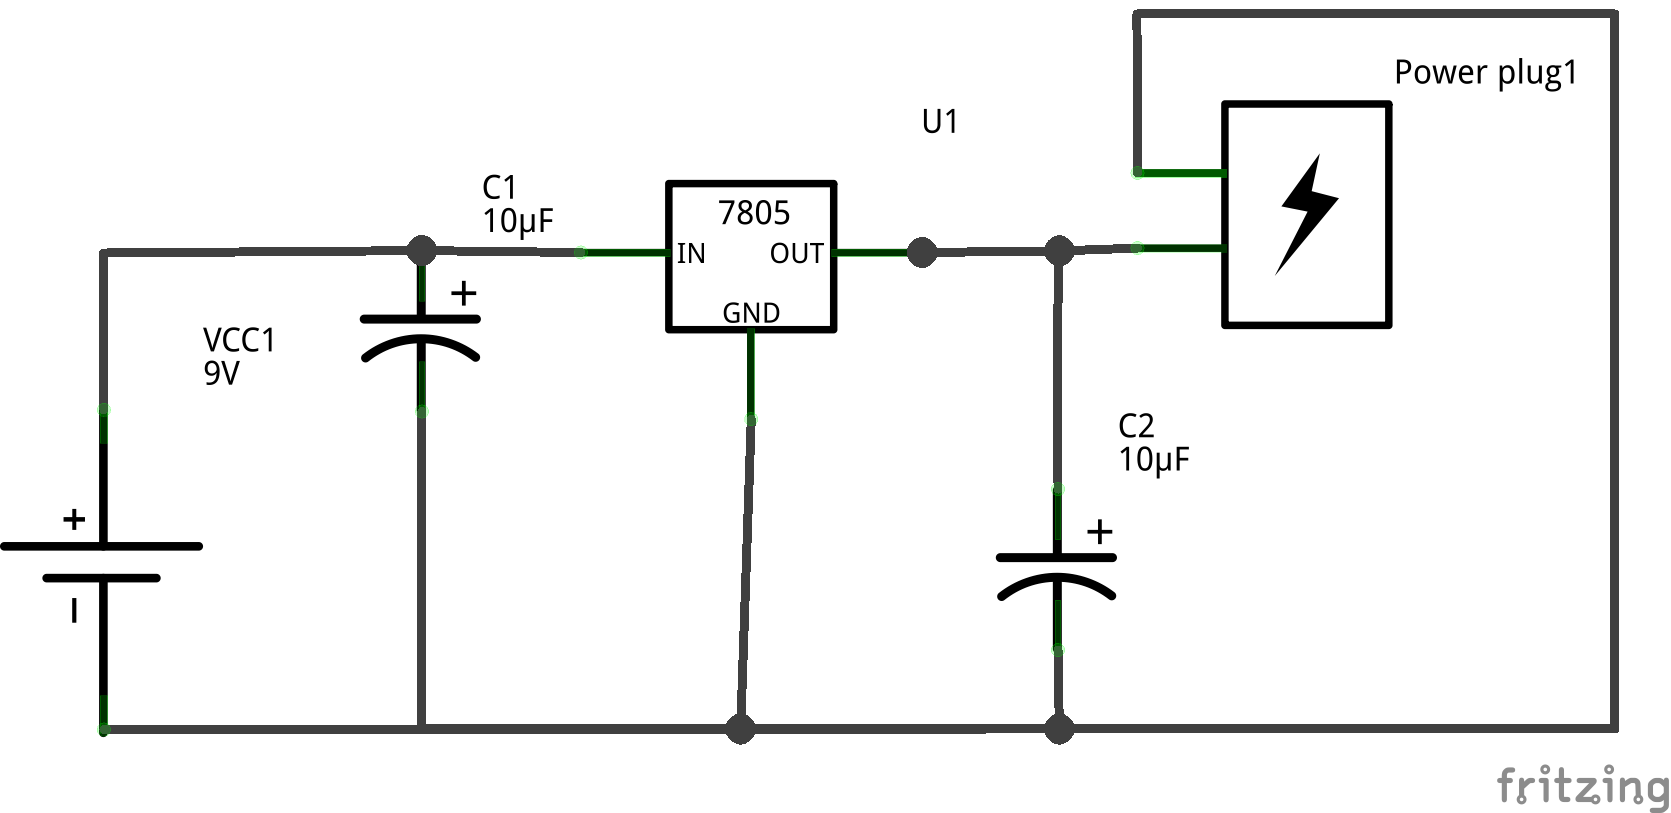
\includegraphics[width=4cm, height=4cm]{img/esquematrans.png}  & 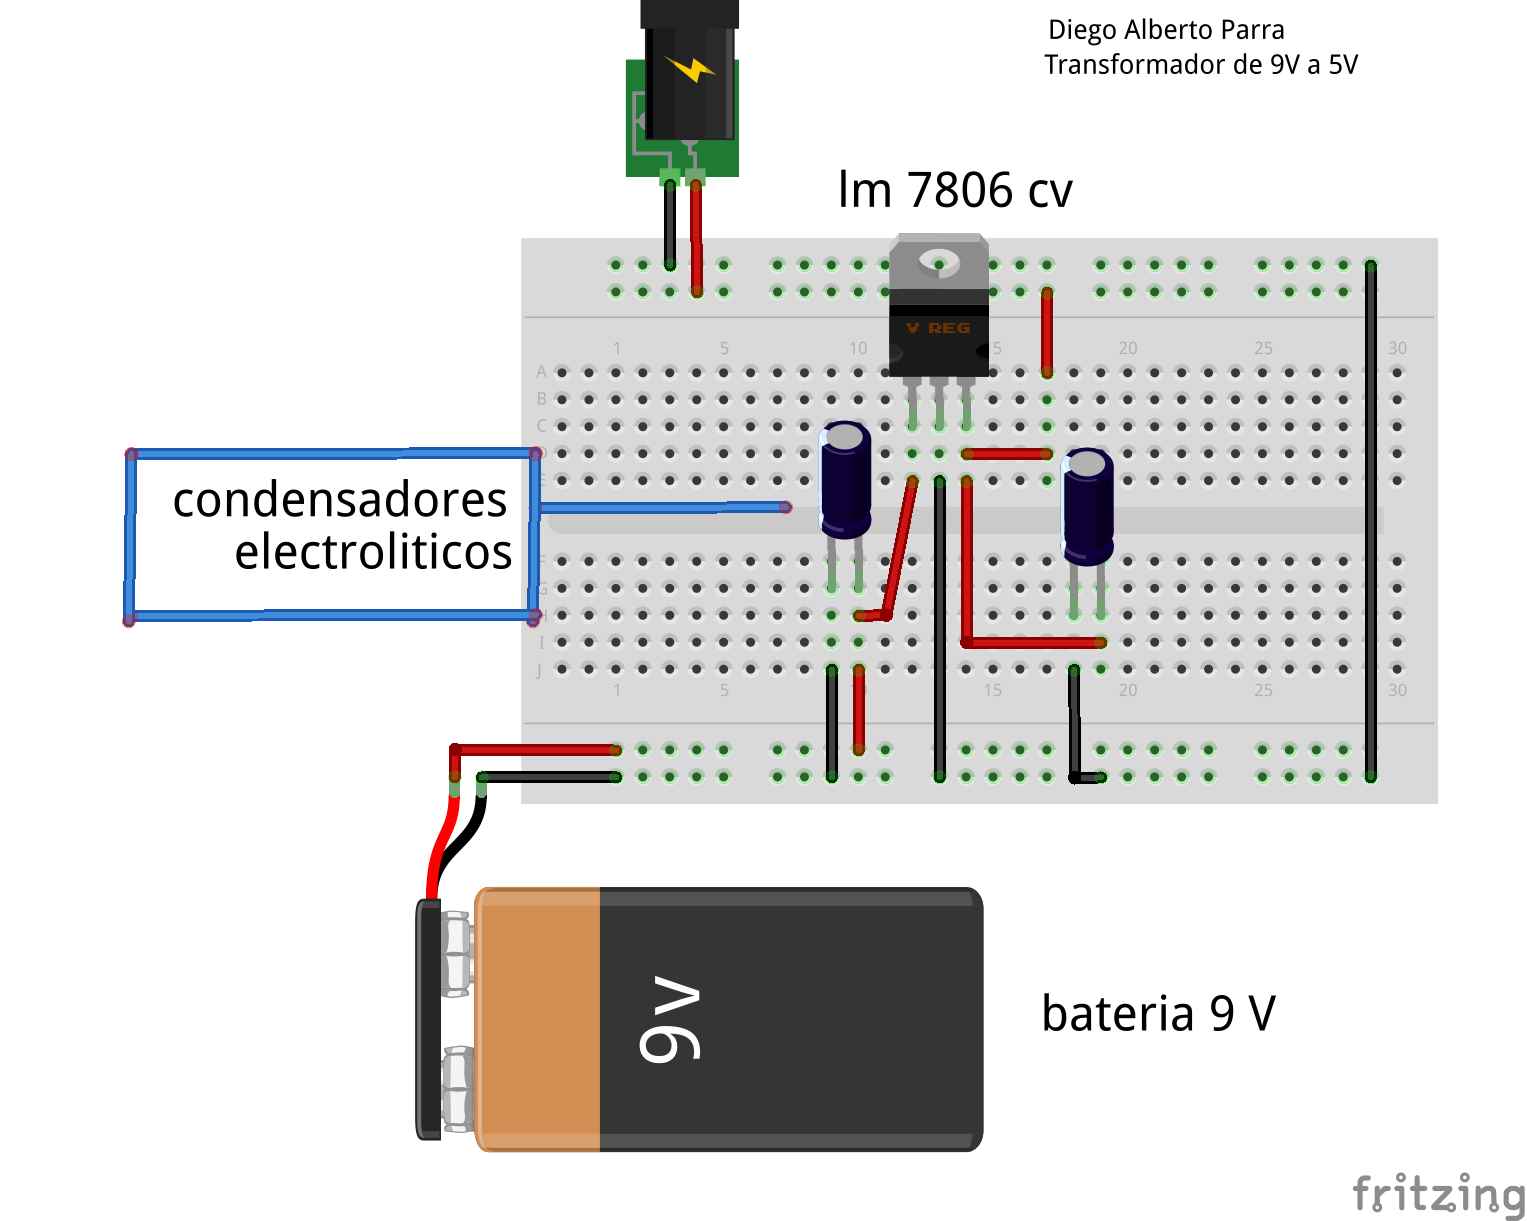
\includegraphics[width=4.cm, height=4cm]{img/montajetr5V.png} \\ \hline
1.A & 1.B \\ \hline
\end{tabular}
\captionof{figure}{Figura 1.A Esquema eléctrico de un transformador \cite{REGULADOR} de 9V a 5V, utilizando transistor lm 7805 cv, con capacitores electrolíticos de 10 microfaradios.  Figura 1.B Montaje en protoboard del circuito.}
\label{fig:g1}
\end{Figure}

\subsubsection{Modulo bluetooth}
El modulo bluetooth se debe conectar de la siguiente manera: el pin 2 de la tarjeta arduino es el Rx, este va conectado al Tx del bluetooth, el pin 3 del microcontrolador es el Tx y va conectado al pin Rx del bluetooth, como se muestra en la figura 2.A y 2.B , conectar el GND del bluetooth al pin 8  o 16 del microcontrolador, ahora conectar el pin de Vcc del bluetooth al pin 7 o 14 del microcontrolador.

\begin{Figure}
\center
\begin{tabular}{|l|r|}
\hline
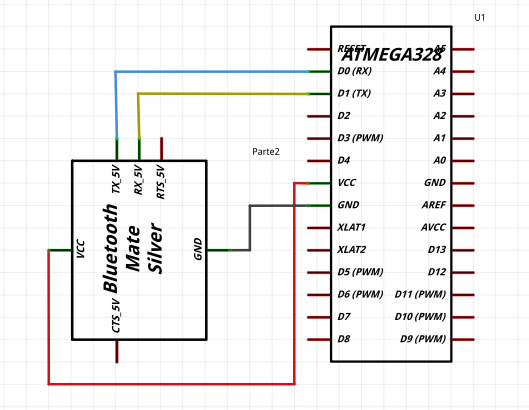
\includegraphics[width=4cm, height=4cm]{img/bluetoothesq.png} & 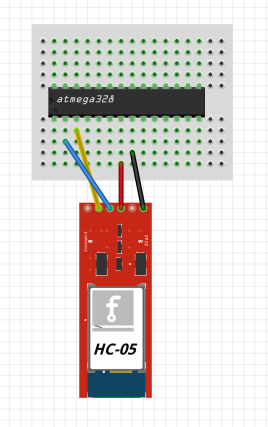
\includegraphics[width=4cm, height=4cm]{img/bluetoothmon.png} \\ \hline
2.A & 2.B \\ \hline
\end{tabular}
\captionof{figure}{Figura 2.A Circuito eléctrico del bluetooth conectado a un microcontrolador atmega 328 P-PU. Figura 2.B Montaje en protoboard, los cables negros son tierra, los cables rojos son voltaje, y los cables de colores son conexiones.}
\label{fig:g2}
\end{Figure}

\subsubsection{Oscilador}
Es necesario olocar un oscilador de 16 mHz el cual se deja siempre en el microcontrolador, esto  con el fin de ajustar los tres relojes internos que trae el integrado atmega 328 P-Pu, para esto se utiliza el cristal de 16 mHz junto con los dos condensadores cerámicos de 12 picofaradios como se muestra en las figuras 3.A y 3.B, uno de los pines del cristal se conecta al pin 9 del microcontrolador y el otro extremo del cristal al pin 10, unir un capacitor a cada extremo del cristal y estos al pin 8 o 16 del microcontrolador de tal forma que los capacitores quedan en paralelo.\\

\begin{Figure}
\center
\begin{tabular}{|l|r|}
\hline
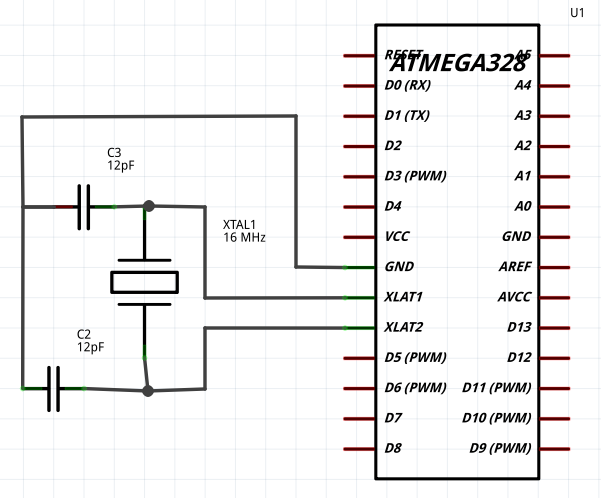
\includegraphics[width=4cm, height=4cm]{img/oscilaesq.png} & 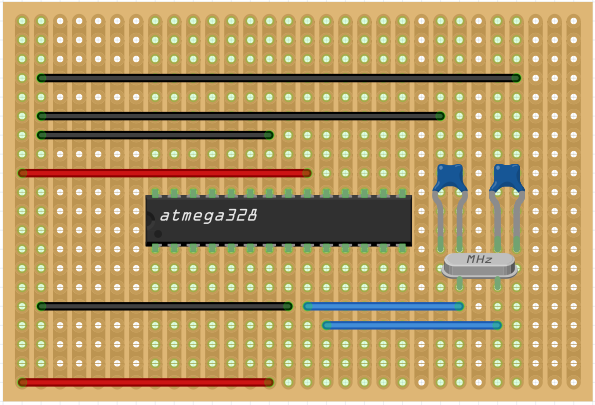
\includegraphics[width=4cm, height=4cm]{img/oscilapro.png} \\ \hline
3.A & 3.B \\ \hline
\end{tabular}
\captionof{figure}{Figura 3.A Esquema circuito eléctrico cristal 16 Mhz, conectado al microcontrolador atmega 328 P-PU. Figura 3.B Montaje en protoboard, los cables negros son tierra, los cables rojos son voltaje, y los cables de colores son conexiones.}
\label{fig:g3}
\end{Figure}

\subsubsection{Botón reset}
Se conecta un  botón como se muestra en la figuras 4.A y 4.B, para reiniciar el  microcontrolador, se une cualquiera de los  extremos del botón al pin 1 del microcontrolador que es el pin de reset, el otro extremo del botón se coneca  a una resistencia de 1 $K\Omega $ y el extremo de la resistencia a tierra.\\

\begin{Figure}
\center
\begin{tabular}{|l|r|}
\hline
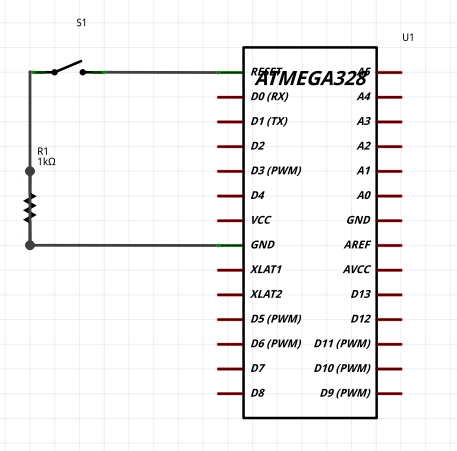
\includegraphics[width=4cm, height=3cm]{img/botonesq.png} & 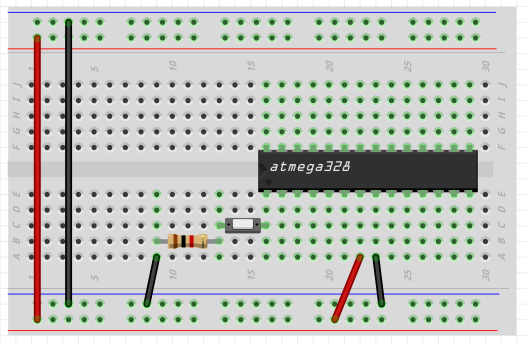
\includegraphics[width=4cm, height=3cm]{img/botonpro.png} \\ \hline
4.A & 4.B \\ \hline
\end{tabular}
\captionof{figure}{Figura 4.A Esquema conexión botón y microcontrolador atmega 328 P-PU. Figura 4.B Montaje en protoboard, los cables negros son tierra, los cables rojos son voltaje.}
\label{fig:g4}
\end{Figure}


\subsubsection{Tip 122 y motor}
Conectar el motor y un sistema de transmisión como se aprecia en la figura 5; se utiliza un transistor tip\cite{TIP122} 122, las conexiones del transistor se muestran en la  figuras 6.A y 6.B.

Conectar una resistencia de 1 $k \Omega $ al pin base del transistor y el otro extremo de la resistencia\footnote{Esto con el fin de limitar la corriente de saturación que llega al pin  base del TIP122 que es de 2 mA a 20 mA, pues el pin PWM del integrado atmega 328 ofrece de 0 a 40 mA de salida.}  unido al pin numero 5 del integrado atmega328P-PU, luego conectar el pin del colector del tip122 a +5V, conectar un  diodo\footnote{El cual se encargara de limitar la corriente en caso de retornar por el colector del transistor hacia tierra cuando el motor se detenga.} regulador entre el colector y uno de los extremos del motor; unir el pin emisor del transistor  al extremo libre del motor y estos dos a tierra; ahora se conecta el condensador cerámico entre los dos pines del motor, como se observa en las  figuras 6.A y 6.B.


\begin{Figure}
\center
\begin{tabular}{|l|r|}
\hline
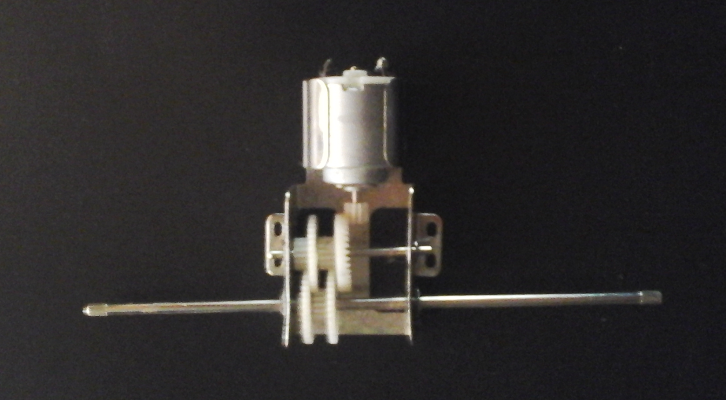
\includegraphics[width=8cm, height=4cm]{img/transmision.png}  \\ \hline
\end{tabular}
\captionof{figure}{Motor con sistema de transmisión para el montaje.}
\label{fig:g5}
\end{Figure}

\begin{Figure}
\center
\begin{tabular}{|l|r|}
\hline
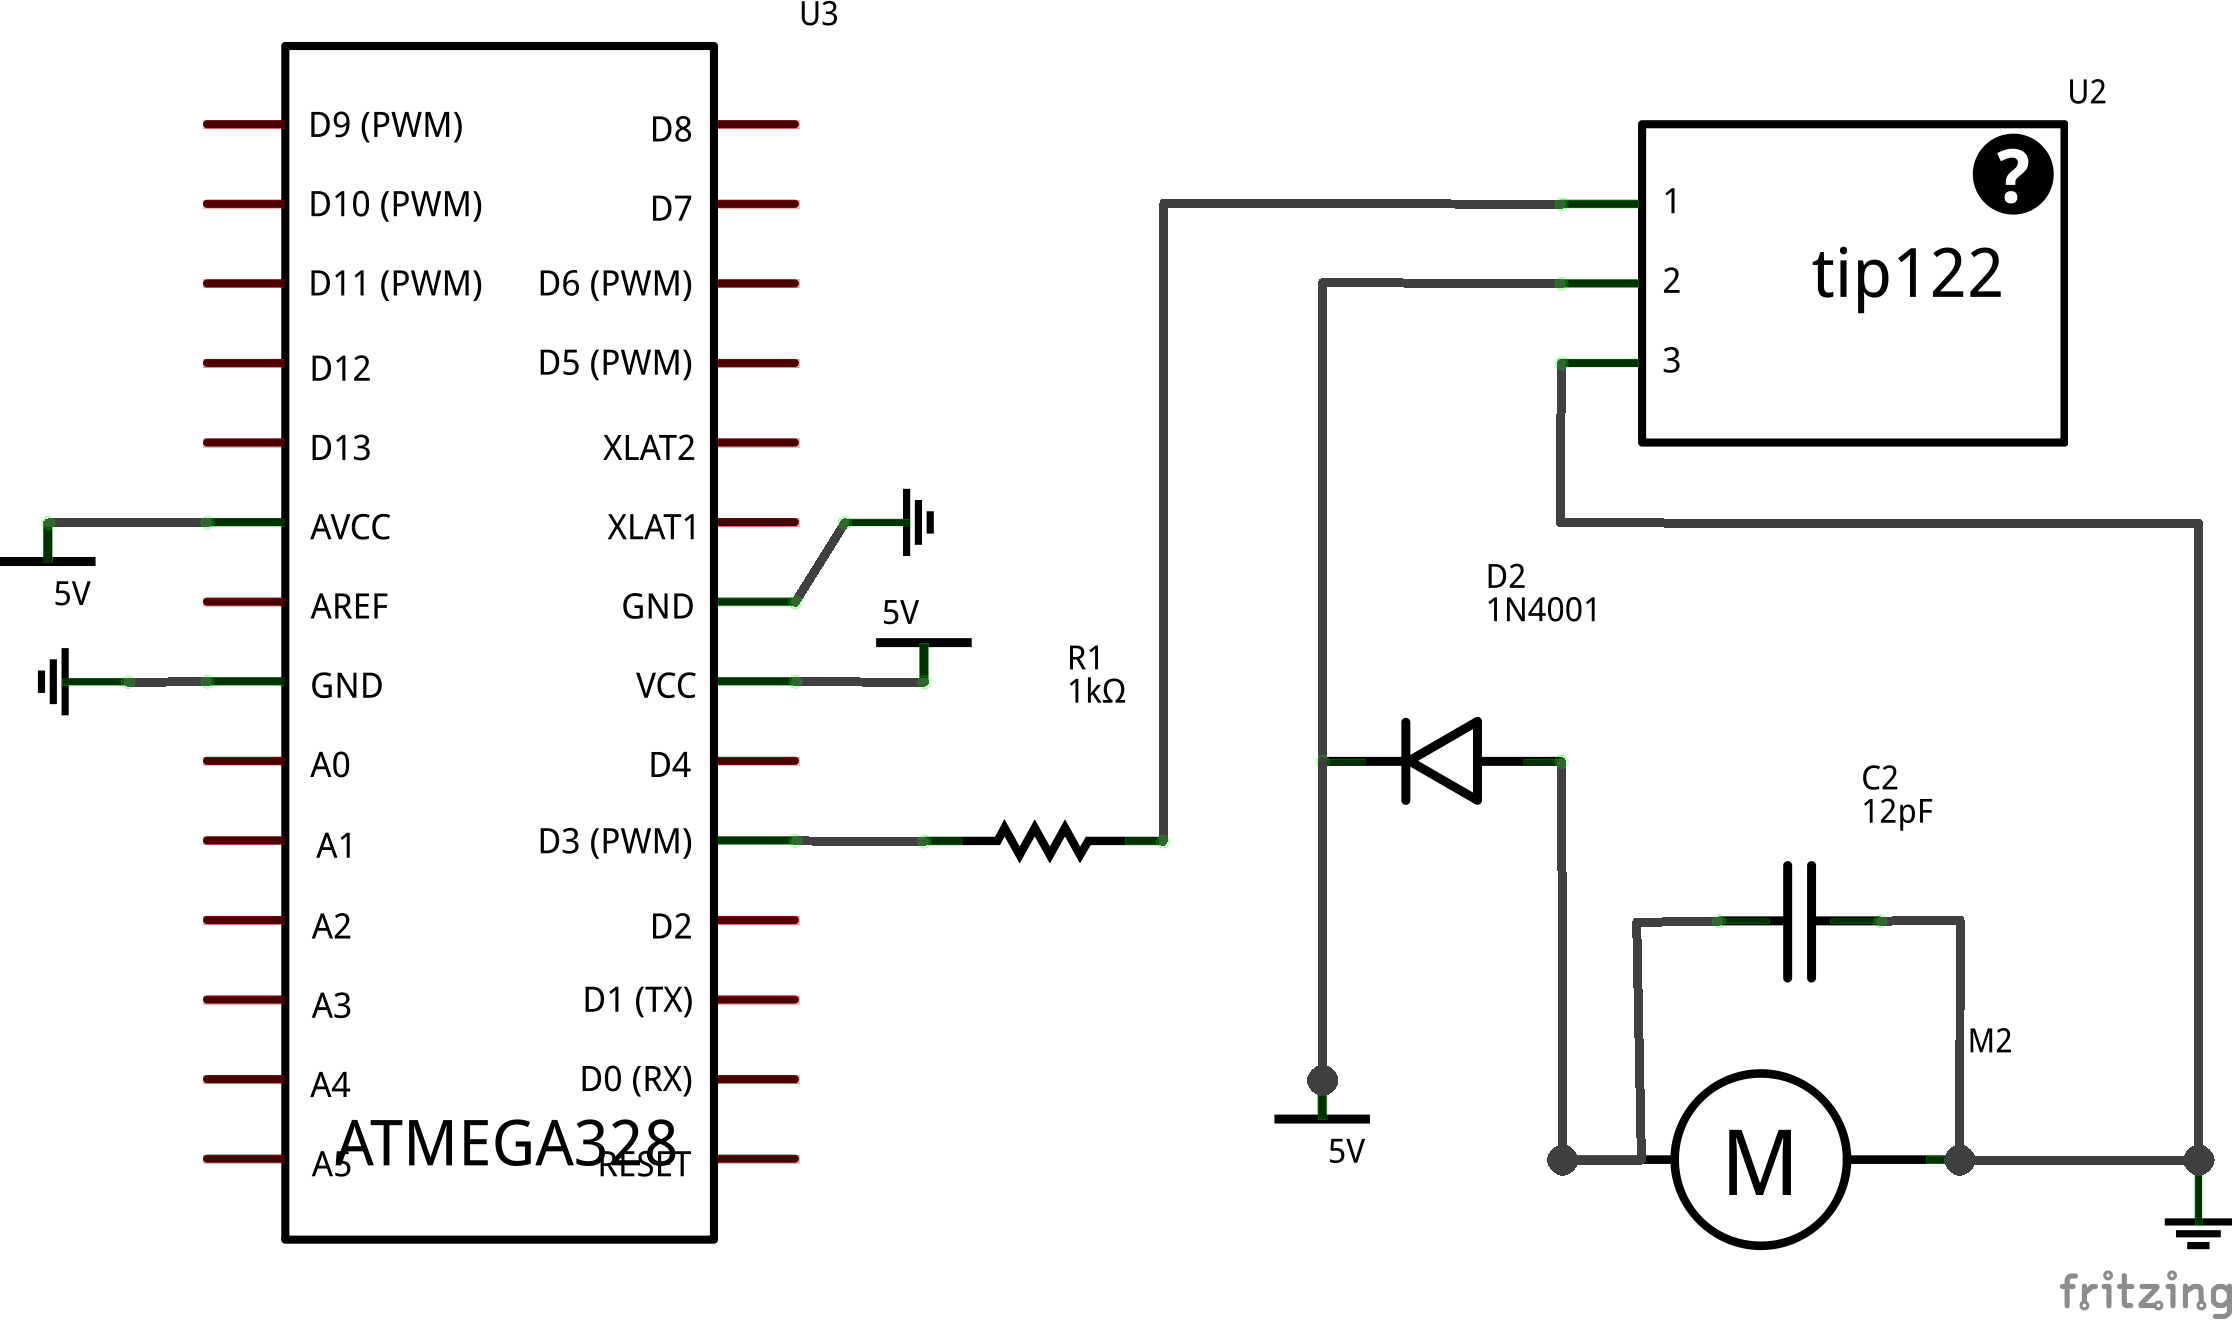
\includegraphics[width=4cm, height=3cm]{img/esquemamotor.png} & 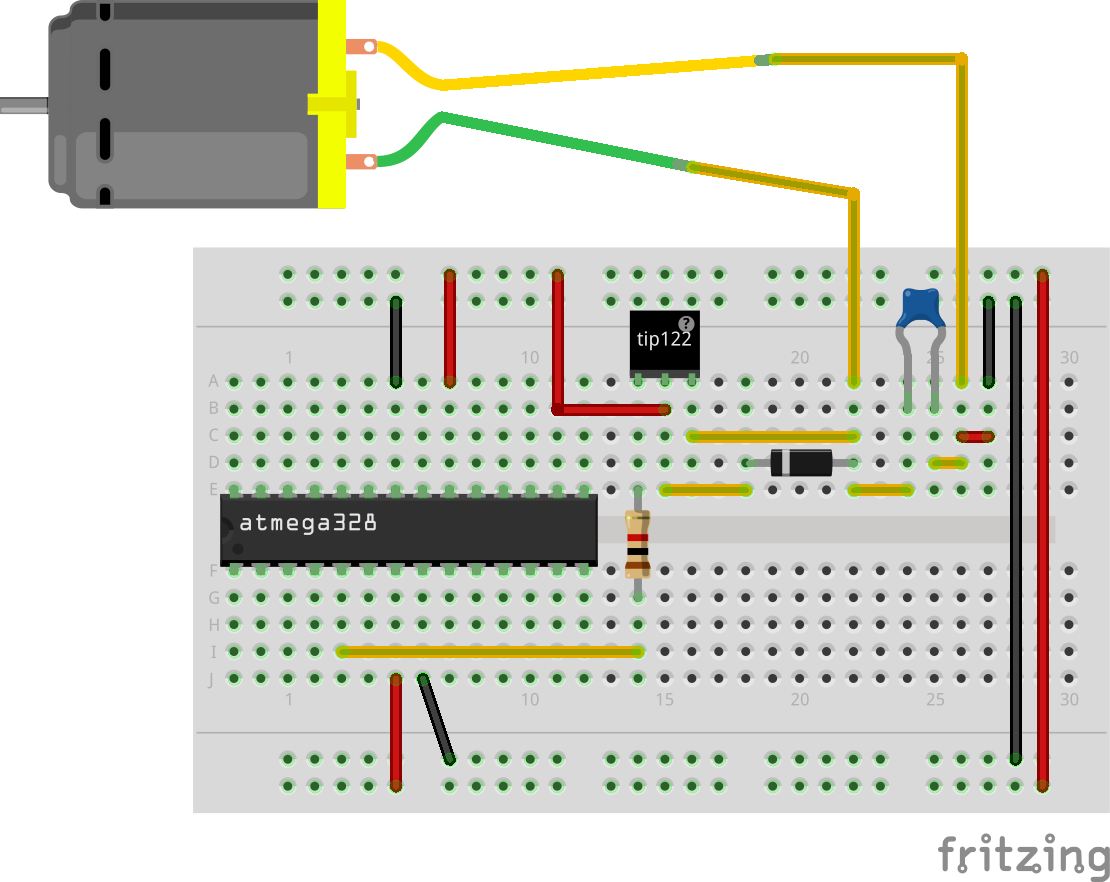
\includegraphics[width=4cm, height=3cm]{img/montajemot.png} \\ \hline
6.A. & 6.B. \\ \hline
\end{tabular}
\captionof{figure}{Figura 6.A Montaje eléctrico del motor conectado al microcontrolador, el tip 122, un diodo regulador, un capacitor cerámico de  12 pF y  resistencia de 1 Komhs. Figura 6.B Montaje en protoboard, los cables negros son tierra, los cables rojos son voltaje, y los cables naranjas son conexiones.}
\label{fig:g6}
\end{Figure}

\subsubsection{Sensor receptor lateral}
Las conexiones del sensor receptor lateral, el cual es un diodo led receptor de luz infrarroja \cite{INFRARED}; se conecta una resistencia de $3 k\Omega$ al ánodo del led y el otro extremo de la resistencia a tierra, luego se conecta el cátodo del led a $+5V$, el pin 23 \footnote{Este pin es la entrada analógica numero cero del microcontrolador atmega.} del microcontrolador se conecta  en un punto intermedio entre la resistencia y el ánodo del diodo led. Como se observa en la figura 7.A y 7.B.

\begin{Figure}
\center
\begin{tabular}{|l|r|}
\hline
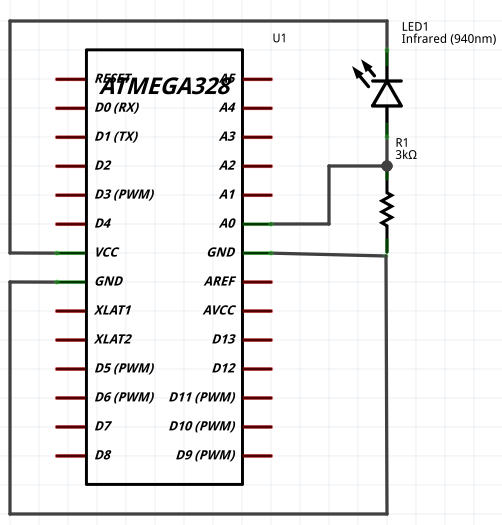
\includegraphics[width=4cm, height=3cm]{img/senlaesq.png} & 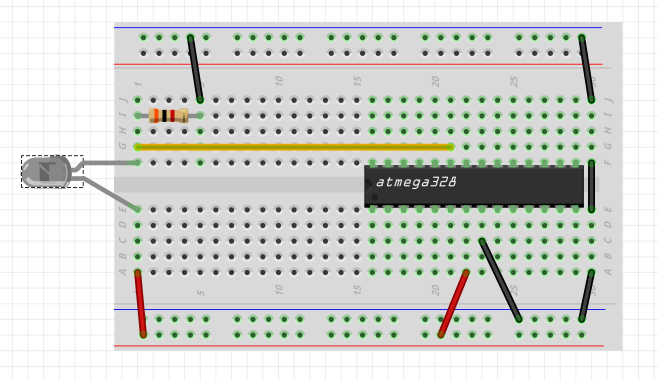
\includegraphics[width=4cm, height=3cm]{img/senlapro.png} \\ \hline
7.A. & 7.B. \\ \hline
\end{tabular}
\captionof{figure}{Figura 7.A Montaje eléctrico del sensor lateral infrarrojo conectado a tarjeta atmega 328 P-PU, con una resistencia de $3 k\Omega$. Figura 7.B Montaje en protoboard, los cables negros son tierra, los cables rojos son voltaje, y los cables naranjas son conexiones.}
\label{fig:g7}
\end{Figure}


\subsubsection{Sensor frontal emisor - receptor}
Las conexiones del sensor receptor frontal, se aprecia en la figura 8.A. y en la figura 8.B; conectar una resistencia de $3 k\Omega$ al ánodo del led receptor y el otro extremo de la resistencia a tierra, luego unir el pin 28 \footnote{Este pin es la entrada analógica numero cinco del microcontrolador atmega.} del microcontrolador en un punto intermedio entre la resistencia y el ánodo del diodo led receptor, el cátodo del diodo receptor se conecta a +5V.\\

Para la  fuente emisora de fotones infrarrojos o radiación infrarroja, se utiliza un diodo led emisor infrarrojo, el cátodo del diodo se une  a la resistencia de $500 \Omega$ y el otro extremo de la resistencia a tierra, el ánodo del diodo se conecta al pin 12\footnote{Salida D6 PWM.} del microcontrolador.\\

\begin{Figure}
\center
\begin{tabular}{|l|r|}
\hline
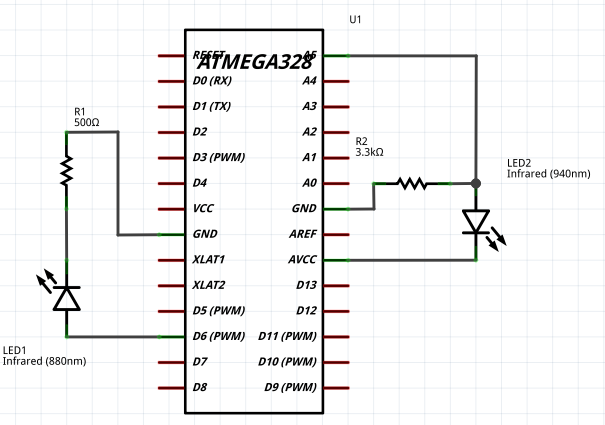
\includegraphics[width=4cm, height=4cm]{img/ledesq.png} & 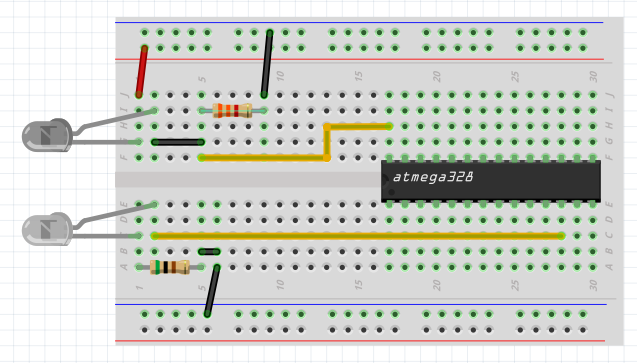
\includegraphics[width=4cm, height=4cm]{img/ledmont.png} \\ \hline
8.A & 8.B \\ \hline
\end{tabular}
\captionof{figure}{Figura 8.A Conexiones de los diodos receptor y emisor con microcontrolador atmega328P-PU. Figura 8.B Montaje en protoboard del sistema emisor receptor infrarrojo, junto a dos resistencias, y el microcontrolador, los cables negros son tierra, los cables rojos son voltaje, el cable naranja son conexiones.}
\label{fig:g8}
\end{Figure}

\subsubsection{Diodo led RGB}
Se utilizan tres diodos led de distintos colores o un diodo led rgb, con el fin de identificar el proceso que esta realizando el microcontrolador y sus diferentes sensores a través del titileo de los led's.
Las conexiones se aprecian en los esquemas de la figura 9.A y 9.B;  el ánodo del diodo rgb se conecta a +5V, el pin rojo del diodo rgb se conecta a una resistencia de $500\Omega$ y el otro extremo de la resistencia se conecta al pin 18 del microcontrolador, el pin verde del diodo rgb unido a una resistencia de $500\Omega$ y el otro extremo de la resistencia se conecta al pin 16 del microcontrolador, el pin azul del diodo se une a una resistencia de $500\Omega$ y el otro extremo de la resistencia se conecta al pin 15 del microcontrolador.\\

\begin{Figure}	
\center
\begin{tabular}{|l|r|}
\hline
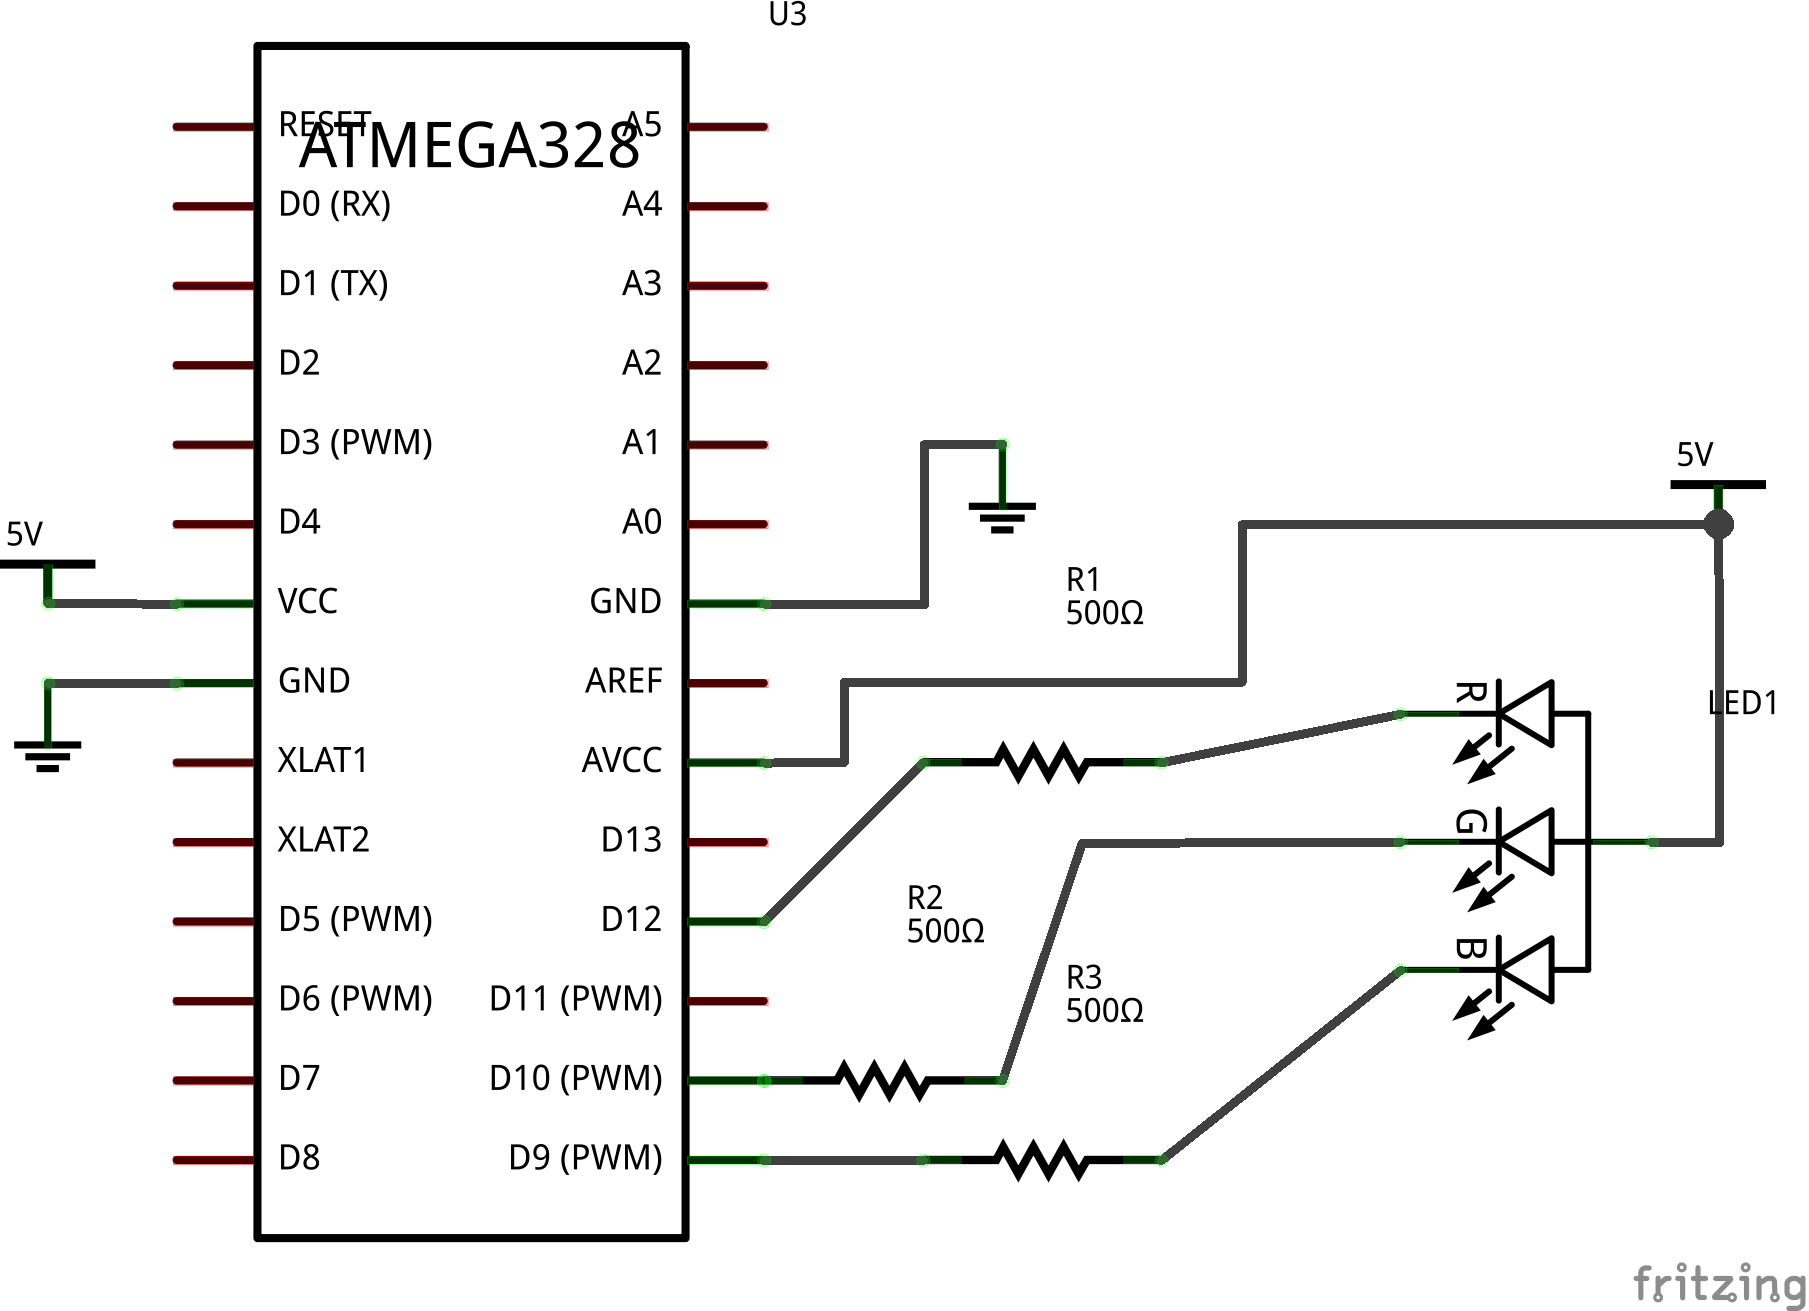
\includegraphics[width=4cm, height=3cm]{img/rgbesq.png} & 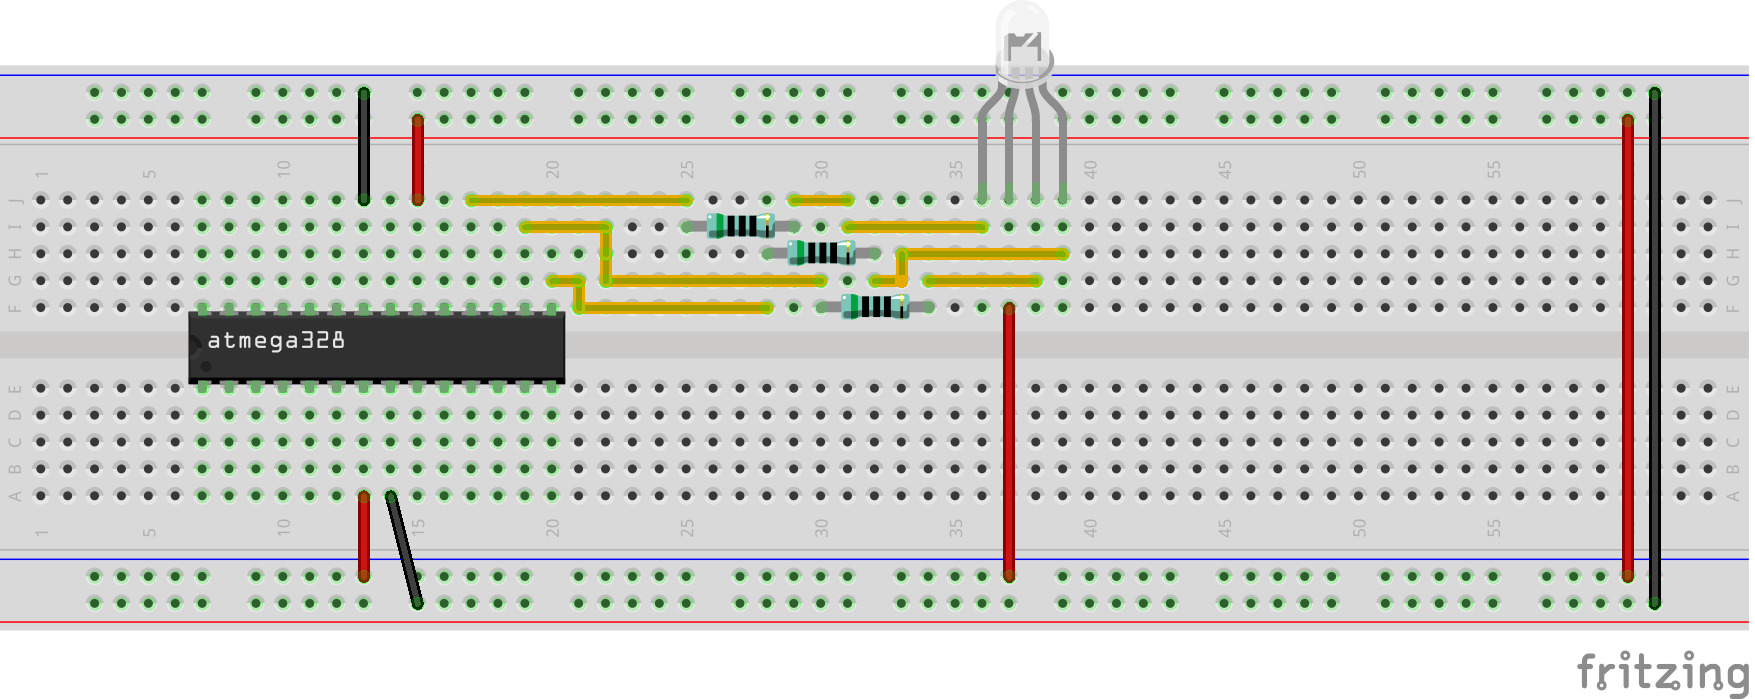
\includegraphics[width=4cm, height=3cm]{img/rgbmont.png} \\ \hline
9.A & 9.B \\ \hline
\end{tabular}
\captionof{figure}{Figura 9.A Circuito eléctrico diodo rgb con el microcontrolador atmega 328 P-PU. Figura 9.B Esquema  del diodo rgb en protoboard.}
\label{fig:g9}
\end{Figure}
\vspace{0.6 cm}

El montaje final de los componentes eléctricos en protoboard y el esquema eléctrico final se encuentran en los anexos A.1 y A.2.
El montaje mecánico se encuentra en los anexos B.1, B.2,  B.3, B4 y B5.

\section{Control de hardware a través del software free infrarossi}

\subsection{¿Qué es free infrarossi?}
Free infrarossi es un  programa creado en Colombia, en la ciudad de Bogotá; el cual fue desarrollado con software libre y en un entorno libre como lo es GNU-Linux, no es multiplataforma, fue diseñado únicamente para este sistema operativo; se vale de lenguajes de programación, como  C, C++, python 2.7, bash; y de programas como arduino, octave, latex, gnuplot, blueman-manager entre otros, fusionados en una interfaz amigable y fácil de utilizar. \\\\
Free infrarossi es un instrumento de laboratorio que ilustra  la propiedad de difracción, atenuación y absorción de ondas electromagnéticas en el espectro infrarrojo, esta diseñado para ser utilizado tanto por  estudiantes como docentes de muy diversas ramas de las ciencias y  la ingeniería o como una herramienta muy útil para los educadores y alumnos de media vocacional.

\subsection{Licencia}
Programa de control de hardware e ilustración física de las propiedades de las ondas electromagnéticas en el espectro infrarrojo.\\
Copyright (C) 2016-01-01  Universidad Distrital Francisco Jose, Dr. Julian Andres Salamanca Bernal, Diego Alberto Parra Garzón. \\
El programa free infrarossi es software libre; puedes redistribuirlo y / o modificarlo bajo los términos de la Licencia Pública General GNU publicada por la Fundación para el Software Libre; ya sea 	la versión 3 de la Licencia, o (a su elección) cualquier versión posterior. \\
Este programa se distribuye con la esperanza de que sea útil, pero SIN NINGUNA GARANTÍA; ni siquiera la garantía implícita de COMERCIALIZACIÓN o IDONEIDAD PARA UN PROPÓSITO PARTICULAR. Vea la Licencia Pública General GNU para más detalles. \\
Debería haber recibido una copia de la Licencia Pública General de GNU junto con este programa; si no, escriba a la Free Software Foundation, Inc., 51 Franklin Street, Quinto Piso, Boston, MA 02110-1301 EE.UU..\\
Si usted hace alguna modificación en esta aplicación, deberá siempre mencionar el autor original de la misma.

\subsection{Instalación}
La instalación de este software es relativamente sencilla, el proceso de instalación es el mismo para distribuciones basadas en Debian\footnote{Pagina oficial proyecto Debian https://www.debian.org/} se  explicara paso a paso el proceso de instalación:
\begin{enumerate}
\item[a.] Abrir una terminal\footnote{Enlace que explica ese procedimiento: http://www.comoinstalarlinux.com/como-abrir-una-terminal-en-ubuntu-linux-mint-centos-debian/} y escribir en ella lo siguiente sin comillas $"$sudo su$"$ y luego oprimir la tecla enter.
\item[b.] Escribir la contraseña de administrador y presione enter; tenga en cuenta que la terminal no muestra la contraseña.
\item[c.] Escriba en la terminal sin comillas $"$aptitude install -y git$"$, presione enter.
\item[d.] Escriba en la terminal sin comillas $"$cd Documentos$"$ presione enter.
\item[e.] Escriba en la terminal sin comillas $"$git clone https://github.com/Diego-debian/Free-infrarossi$"$, presione enter.
\item[f.] Escriba en la terminal sin comillas $”$chmod +777 Free-infrarossi$”$, presione la tecla enter.
\item[g.] Cierre la terminal y diríjase al navegador de archivos o gestor de archivos y ábralo.
\item[h.] Diríjase a la carpeta Documentos/Free-infrarossi/\\install.
\item[j.] Hacer click derecho con el mouse en el archivo instalador.py,  dar click izquierdo en propiedades; en la pestaña de general debe decir abrir archivo con python 2.7 y en la pestaña permisos debe estar seleccionada la casilla permitir ejecutar este archivo como programa, de no ser así cambie las opciones y déjelas como se menciono antes.
\item[k.] Cierre la ventana y abra el archivo INSTALADOR.py haciendo doble click izquierdo sobre este.
\item[l.] Escriba su contraseña de administrador y presione enter.
\item[m.] Una vez abierto el instalador escriba  1 y presione enter.
\item[n.] Escriba nuevamente 1 y enter.
\item[ñ.] Una vez finalizada la instalación se aconseja reinicie su pc.
\end{enumerate}

\subsection{Primer uso free infrarossi}

Una vez este reiniciado el computador, lo primero  es abrir una terminal del S.O. escribir en la terminal sin comillas $'infrarossi'$ y oprimir la tecla enter, escribir la clave de administrador y se abrirá la ventana del software free infrarossi, como se aprecia en la figura 10.
\begin{Figure}	
\center
\begin{tabular}{|l|r|}
\hline
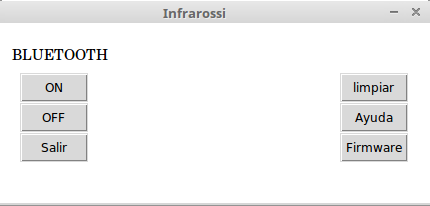
\includegraphics[width=8cm, height=4cm]{img/infrarossi.png} \\ \hline
%10. \\ \hline 
\end{tabular}
\captionof{figure}{Ventana del software free infrarossi}
\label{fig:g10}
\end{Figure}


\subsection{Carga de firmware en integrado atmega 328}
En la ventana del programa free infrarossi, en la parte inferior derecha hay tres botones, oprimir el botón de firmware y conectar la tarjeta micro controladora arduino uno al pc; acto seguido oprimir el botón continuar y esperar que cargue el firmware en la tarjeta, una vez hecho esto retirar el micro controlador de la tarjeta y colocarlo en el montaje del vehículo.
\begin{Figure}	
\center
\begin{tabular}{|l|r|}
\hline
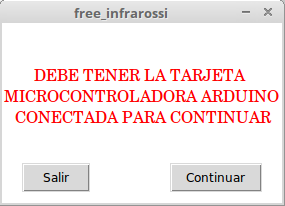
\includegraphics[width=8cm, height=4cm]{img/firmware.png} \\ \hline
%11. \\ \hline
\end{tabular}
\captionof{figure}{Ventana de instalación del firmware, que ofrece el software free infrarossi, para el vehículo motorizado infrarossi.}
\label{fig:g11}
\end{Figure}


\section{Conclusiones}
\begin{enumerate}
\item[*] Las tecnologías libres favorecen la enseñanza y aprendizaje de las ciencias.
\item[*] Con las instrucciones mencionadas anteriormente se consigue un modelo didáctico, muy practico  e interesante capaz de ser muy funcional y de bajo costo.
\item[*] El uso de software y hardware libre es una herramienta que no se puede dejar a un lado, pues hace que la enseñanza en ciencias este muy ligada a la parte experimental.
\end{enumerate}

\begin{thebibliography}{99}
\bibitem{ARDUINO} Monk, S. (2013). 30 Arduino projects for the evil genius. McGraw-Hill Professional.
\bibitem{REGULADOR} Semiconductor, F. (2012). LM7805 Data Sheet. [Online]. Disponible en:\\ http://pdf.datasheetcatalog.net/datasheet/fairchild/\\LM7805.pdf
\bibitem{TIP122} Semiconductor, F. (2008). Tip120/tip121/tip122 npn epitaxial darlington transistor. TIP120 datasheet, Oct. [Online]. Disponible en:\\ http://pdf.datasheetcatalog.net/datasheet/fairchild/\\TIP122.pdf.
% \bibitem{DIODO}  Hoja de datos diodo regulador 1N4001. http://pdf.datasheetcatalog.net/datasheet/lrc/\\1N4001.pdf
%\bibitem{INFRARED} Hoja de datos de los diodos led infrarrojos, emisor y receptor. \\ http://www.datasheetarchive.com/dlmain/Datasheets\\-31/DSA-617614.pdf
\bibitem{FRITZING} Knörig, A., Wettach, R., \& Cohen, J. (2009, February). Fritzing: a tool for advancing electronic prototyping for designers. In Proceedings of the 3rd International Conference on Tangible and Embedded Interaction. ACM.
\bibitem{PYTHON} Gift, N., \& Jones, J. M. (2008). Python for Unix and Linux system administration. " O'Reilly Media, Inc.".
\bibitem{CIRCUITOS} Alexander, C. K., Sadiku, M. N., Bermúdez, A. V., \& Pedraza, C. R. C. (2006). Fundamentos de circuitos eléctricos. McGraw-Hill. 

\end{thebibliography}
\end{multicols}

%\clearpage % o \cleardoublepage
\selectlanguage{spanish}
\appendix
\addappheadtotoc
\appendixpage

\section{Esquemas}
\subsection{Montaje final protoboard}
\begin{Figure}	
\center
\fbox{
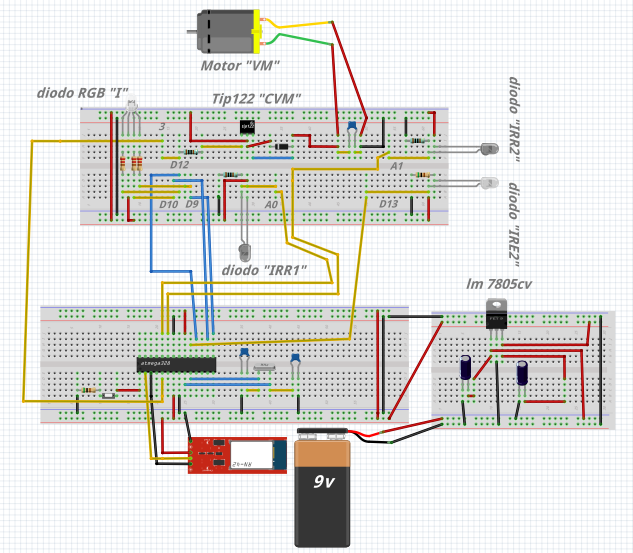
\includegraphics[width=18cm, height=15cm, angle=90]{img/montajep.png} 
	}
\captionof{figure}{Montaje eléctrico final.}
\label{fig:A}
\end{Figure}

\subsection{Circuito eléctrico final.}
\begin{Figure}	
\center
\fbox{
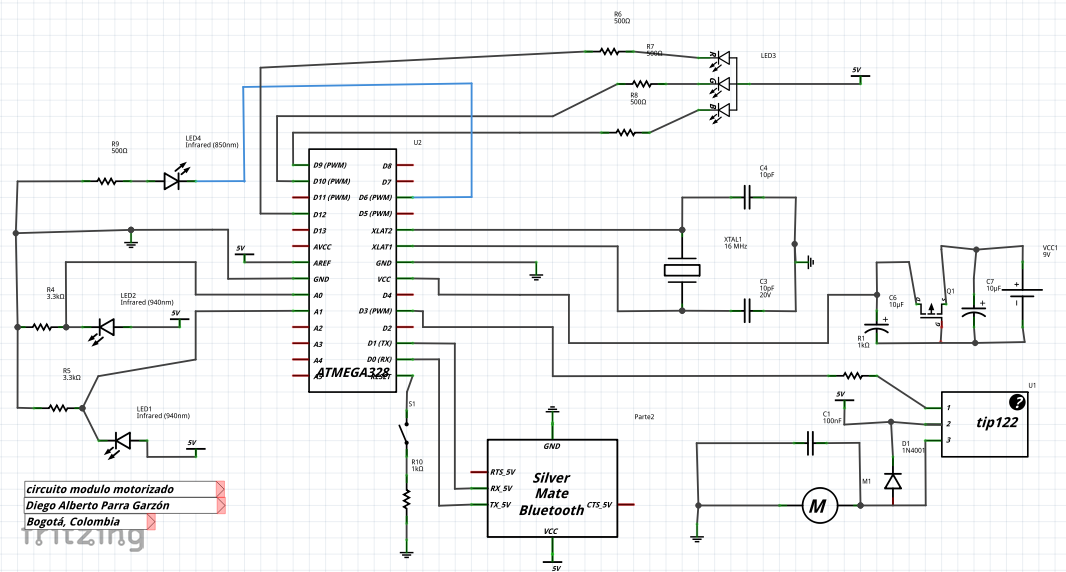
\includegraphics[width=19cm, height=15cm, angle=90]{img/esquemap.png} 
	}
\captionof{figure}{Circuito eléctrico del proyecto.}
\label{fig:B}
\end{Figure}

\section{Chasis}
\subsection{Dimensiones del chasis}
\begin{Figure}	
\center
\fbox{
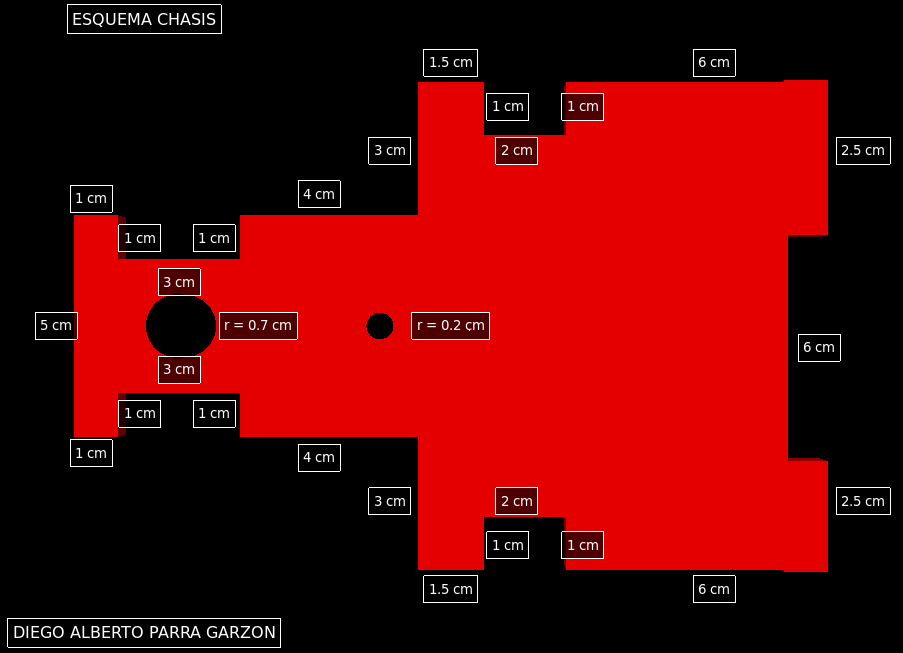
\includegraphics[width=18cm, height=15cm, angle=-90]{img/chasis.png} 
	}
\captionof{figure}{Dimensiones del chasis o base donde reposara el circuito eléctrico, el sistema de transmisión y demas elementos del vehiculo. Figura modelada en python visual.}
\label{fig:C}
\end{Figure}

\subsection{Montaje simulado vista inferior}
\begin{Figure}	
\center
\fbox{
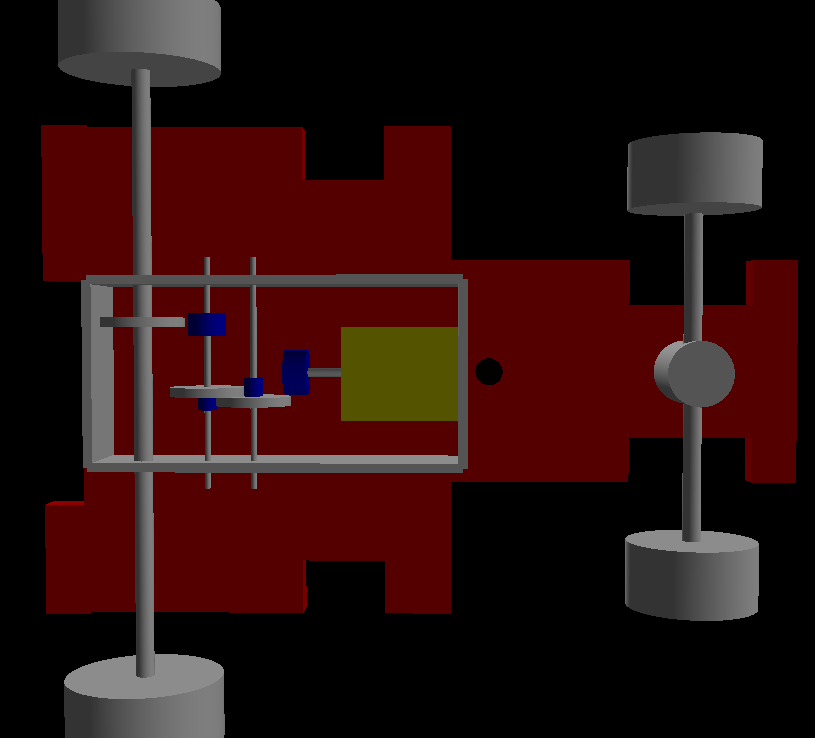
\includegraphics[width=9cm, height=7.5cm, angle=180]{img/montaje2.png} 
	}
\captionof{figure}{Vista inferior del montaje del vehículo con la transmisión y el eje delantero, sin la parte eléctrica. Figura modelada en python visual.}
\label{fig:D}
\end{Figure}


\subsection{Montaje simulado vista superior}
\begin{Figure}	
\center
\fbox{
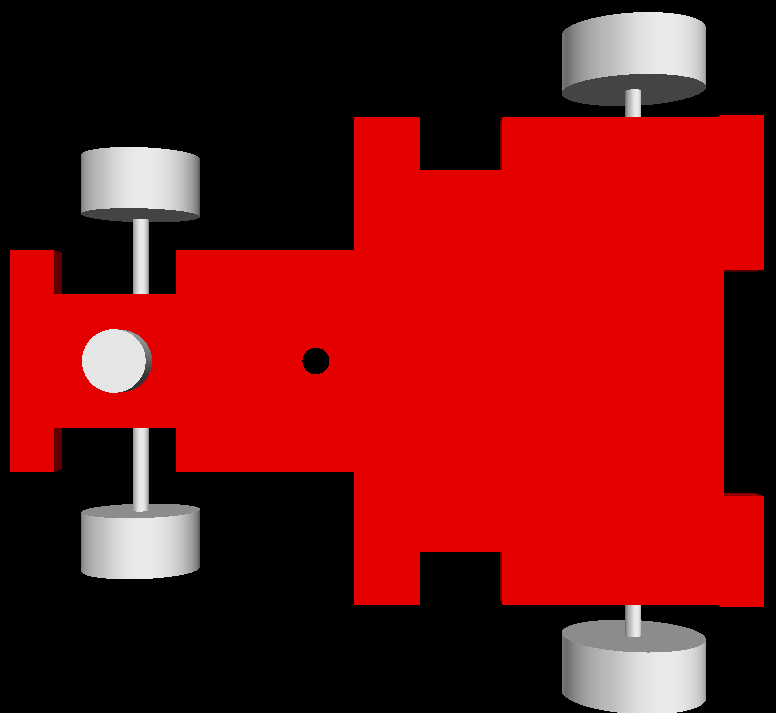
\includegraphics[width=9cm, height=7.5cm, angle=180]{img/montaje1.png} 
	}
\captionof{figure}{Vista superior del montaje del vehículo con la transmisión y el eje delantero, sin la parte eléctrica. Figura modelada en python visual.}
\label{fig:E}
\end{Figure}


\subsection{Montaje real vista inferior}
\begin{Figure}	
\center
\fbox{
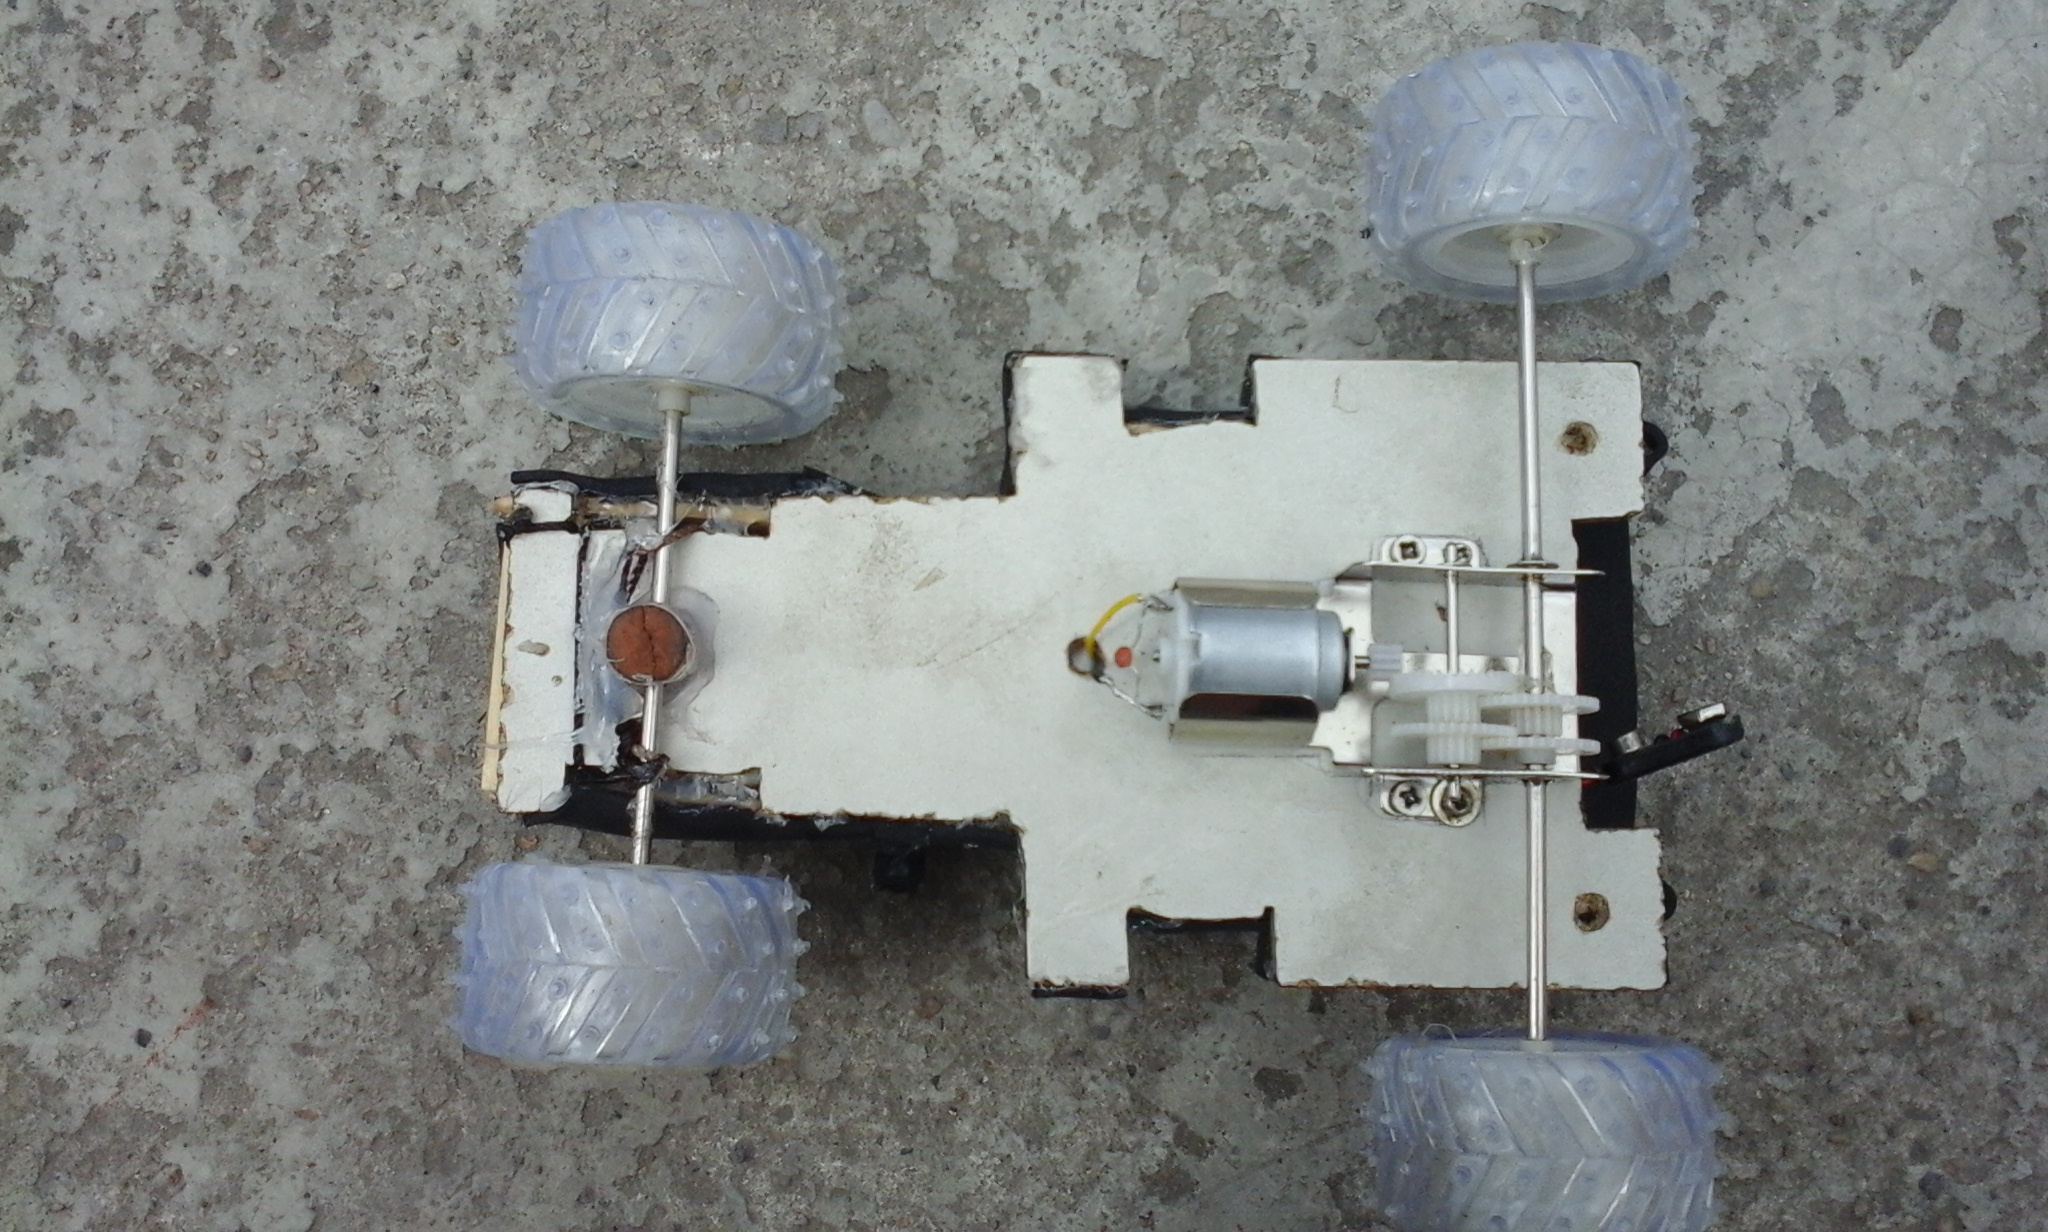
\includegraphics[width=12cm, height=7.5cm, angle=180]{img/monreal2.png} 
	}
\captionof{figure}{Vista inferior del montaje.}
\label{fig:F}
\end{Figure}


\subsection{Montaje real vista superior}
\begin{Figure}	
\center
\fbox{
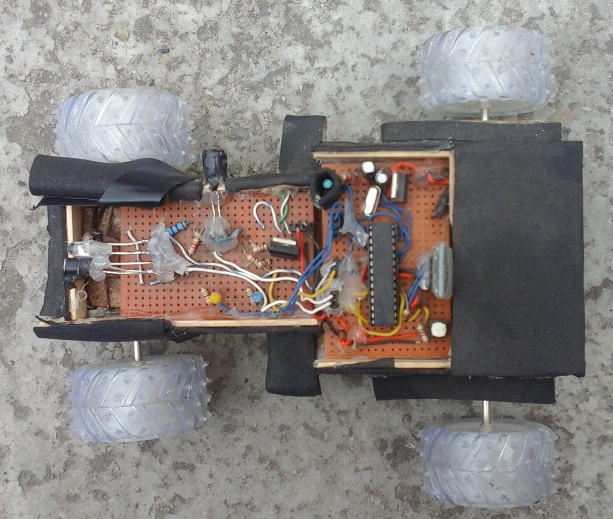
\includegraphics[width=8cm, height=7.5cm, angle=180]{img/monreal3.png} 
	}
\captionof{figure}{Vista superior del montaje.}
\label{fig:G}
\end{Figure}

\subsection{Montaje vista frontal}
\begin{Figure}	
\center
\fbox{
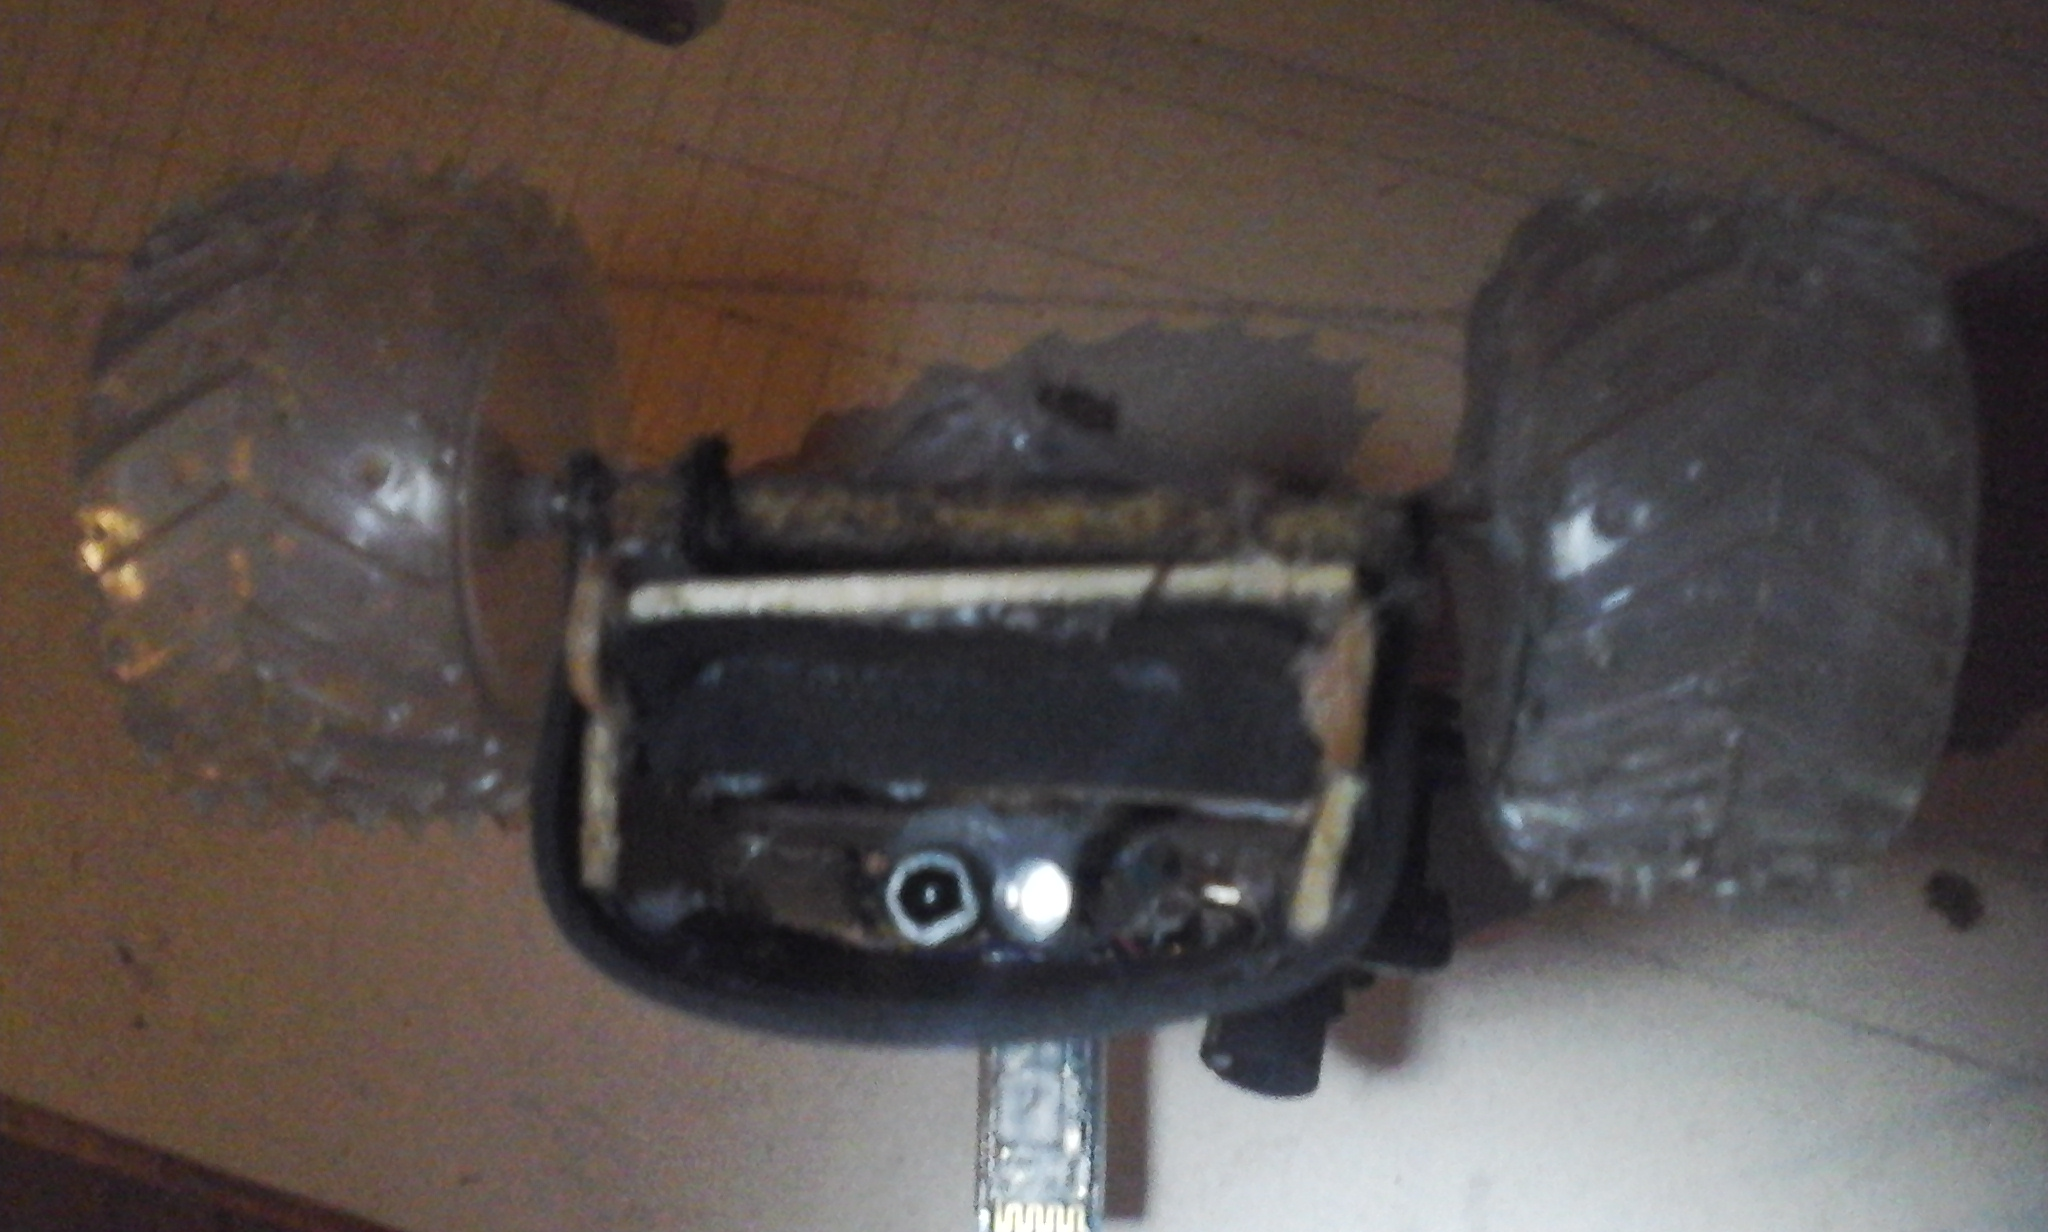
\includegraphics[width=12cm, height=7.5cm, angle=180]{img/vistafront.png} 
	}
\captionof{figure}{Vista frontal montaje.}
\label{fig:H}
\end{Figure}
\end{document}




